\section{Conclusion}


From all these dispersion relations some information can be concluded.
In this section we will give an overview about our findings and formulate some conclusions.


Let us first start by looking at the Dispersion diagram of $ g $ and $ \omega $ as seen in in the lower plot in Figure \ref{fig:DispersionRelations}.
The shape of these curves look complicity differed from the two other graphs.
In fact the dispersion relations are just straight line.
This behaviour is exactly as we would expect, it tells us that the equation are scale invariant, as the parameter $ g $ told us something about the scale of the problem, it gave a dimension to the equations.
The linear relation between the eigenfrequencies and $ g $ means that when $ g $ gets rescaled than the eigenfrequencies are rescaled by the same amount.



The two other dispersion relations in  Figure \ref{fig:DispersionRelations} look very similar is shape, although there is a much greater difference between two neighbour eigenvalues in the $ \sigma $ dispersion relation than for the $ K $ dispersion relation.
Recall that $ \sigma $ was the gradient of the density.
If this gradient becomes larger we would expect the waves to more and more diverge from there sinusoidal shape, this is exactly what we could see when we plot some solutions for increasing $ \sigma $, an example plot can be seen in Figure \ref{fig:IncreasingSig}.


The influence of $ K $ was not entirely clear to me, when we changed the $ K $ value the eigenvalues changed according to the dispersion relation as given in right plot in Figure \ref{fig:DispersionRelations} but the shape of the curve remained the same, so if we changed the value of $ K $  over a curtain range and normalized the solutions all the curves perfectly overlapped each other.
The physical interpretation of this was that $ K $ did not influence the medium in which the wave was propagating and thereby did not influence the shape of the wave.
$ K $ is only a internal parameter to the wave itself and thereby will only influence the eigenfrequencies and the amplitude of the wave, $ K $ is probably directly linked to the energy transported by the wave.


\begin{figure}
\centering
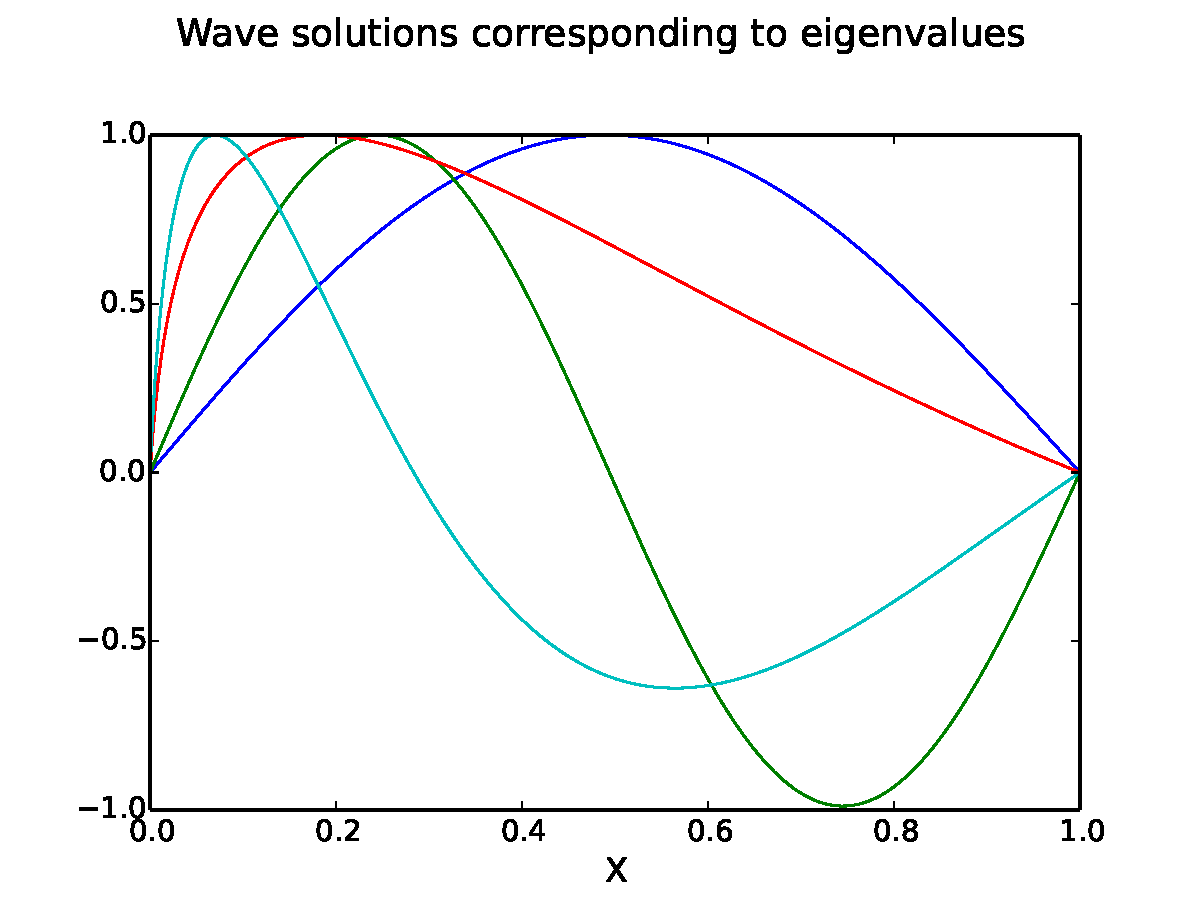
\includegraphics[width=10cm]{../src/plot/IncreasingSig}
\caption{Solutions for the wave equation matching the boundary conditions for increasing $ \sigma $. The dark blue and green curve are for values of $ \sigma $ very close to 0. The other two curves have a larger value for $ \sigma $ and start to diverge more from an ideal sine wave solution.}
\label{fig:IncreasingSig}
\end{figure}
